% Created 2017-05-07 Sun 17:01
% Intended LaTeX compiler: pdflatex
\documentclass[a4paper,11pt]{article}
\usepackage[utf8]{inputenc}
\usepackage[T1]{fontenc}
\usepackage{graphicx}
\usepackage{grffile}
\usepackage{longtable}
\usepackage{wrapfig}
\usepackage{rotating}
\usepackage[normalem]{ulem}
\usepackage{amsmath}
\usepackage{textcomp}
\usepackage{amssymb}
\usepackage{capt-of}
\usepackage{hyperref}
\usepackage[margin=1.2in]{geometry}
\usepackage{setspace}
\onehalfspacing
\usepackage{parskip}
\usepackage{amsthm}
\usepackage{amsmath}
\usepackage{mathtools}
\usepackage{hyperref}
\usepackage{graphicx}
\usepackage{tabularx}
\usepackage{booktabs}
\usepackage{color}
\usepackage{caption}
\usepackage{subcaption}
\hypersetup{colorlinks,citecolor=black,filecolor=black,linkcolor=black,urlcolor=black}
\newtheorem{mydef}{Definition}
\newtheorem{mythm}{Theorem}
\newcommand{\dx}{\mathrm{d}}
\newcommand{\var}{\mathrm{Var}}
\newcommand{\cov}{\mathrm{Cov}}
\newcommand{\corr}{\mathrm{Corr}}
\newcommand{\pr}{\mathrm{Pr}}
\newcommand{\rarrowd}[1]{\xrightarrow{\text{ \textit #1 }}}
\renewcommand\chaptername{Lecture}
\DeclareMathOperator*{\plim}{plim}
\newcommand{\plimn}{\plim_{n \rightarrow \infty}}
\setcounter{secnumdepth}{2}
\author{Zheng Tian}
\date{}
\title{Lecture 9: Hypothesis Tests and Confidence Intervals in Multiple Regression}
\hypersetup{
 pdfauthor={Zheng Tian},
 pdftitle={Lecture 9: Hypothesis Tests and Confidence Intervals in Multiple Regression},
 pdfkeywords={},
 pdfsubject={},
 pdfcreator={Emacs 25.1.1 (Org mode 9.0.3)},
 pdflang={English}}
\begin{document}

\maketitle

\section{Introduction}
\label{sec:org1a8b7d0}

\subsection{Overview}
\label{sec:org5f79219}
This lecture presents the methods for testing the hypotheses
concerning the coefficients in a multiple regression model. Besides
the t-statistic that we have learned in Lecture 6, we introduce a new
test statistic, the F-statistic, which is used to test the joint
hypotheses that involve two or more coefficients. We will also learn
some basic ideas of assessing model specification.


\subsection{Learning goals}
\label{sec:org3b0a59c}
\begin{itemize}
\item Know how to test a hypothesis for a single coefficient using the
t-statistic.
\item Know how to test a joint hypotheses for more than one coefficients
using the F-statistic.
\item Understand the underlying ideas of the F-statistic, especially when
using the homoskedasticity-only F-statistic.
\end{itemize}


\subsection{Reading materials}
\label{sec:org9921d10}
\begin{itemize}
\item Chapter 7 and Section 18.3 in \emph{Introduction to Econometrics} by
Stock and Watson.
\end{itemize}


\section{Hypothesis Tests and Confidence Intervals For a Single Coefficient}
\label{sec:org1fac125}

We consider the general multiple regression model as follows
\begin{equation}
\label{eq:jnt-hyp-mod}
\mathbf{Y} = \beta_0 \boldsymbol{\iota} + \beta_1 \mathbf{X}_1 + \beta_2 \mathbf{X}_2 + \cdots + \beta_k \mathbf{X}_k + \mathbf{u}
\end{equation}
where \(\mathbf{Y}, \mathbf{X}_1, \mathbf{X}_2, \ldots, \mathbf{X}_k, \text{ and } \mathbf{u}\) are \(n
\times 1\) vectors of the dependent variable, regressors, and
errors. \(\boldsymbol{\beta} = (\beta_0, \beta_1, \beta_2, \ldots,
\beta_k)^{\prime}\) is the \((k+1) \times 1\) vector of coefficients. And
\(\boldsymbol{\iota}\) is the \(n \times 1\) vector of 1s.

\subsection{Standard errors for the OLS estimators}
\label{sec:orgb35be3b}

\subsubsection*{A review on \(\var(\hat{\boldsymbol{\beta}}|X)\)}
\label{sec:org3a2b102}

Recall that in the last lecture, we concluded that the the covariance
matrix of the OLS estimators \(\hat{\boldsymbol{\beta}}\) can take the
following forms:

\begin{itemize}
\item The homoskedasticity-only covariance matrix if \(u_i\) is
homoskedastic

\begin{equation}
\label{eq:varbhat-hm-1}
\var(\hat{\boldsymbol{\beta}} | \mathbf{X}) = \sigma^2_u (\mathbf{X}^{\prime} \mathbf{X})^{-1}
\end{equation}

\item The heteroskedasticity-robust covariance matrix if \(u_i\) is
heteroskedastic

\begin{equation}
\label{eq:varbhat-ht-1}
\var_{\mathrm{h}}(\hat{\boldsymbol{\beta}} | \mathbf{X}) = \left(\mathbf{X}^{\prime} \mathbf{X}\right)^{-1} \boldsymbol{\Sigma} (\mathbf{X}^{\prime} \mathbf{X})^{-1}
\end{equation}

where \(\boldsymbol{\Sigma} = \mathbf{X}^{\prime} \boldsymbol{\Omega}
  \mathbf{X}\), and \(\mathbf{\Omega} = \var(\mathbf{u} |
  \mathbf{X})\).
\end{itemize}

Also, we know that if the least squares assumptions hold,
\(\hat{\boldsymbol{\beta}}\) has an asymptotic multivariate normal
distribution as

\begin{equation}
\label{eq:normal-bhat-m}
\hat{\boldsymbol{\beta}} \rarrowd{d} N(\boldsymbol{\beta}, \mathbf{\Sigma_{\hat{\boldsymbol{\beta}}}})
\end{equation}

where \(\mathbf{\Sigma_{\hat{\boldsymbol{\beta}}}} =
\var(\hat{\boldsymbol{\beta}} | \mathbf{X})\) for which use
Equation (\ref{eq:varbhat-hm-1}) for the homoskedastic case and Equation
(\ref{eq:varbhat-ht-1}) for the heteroskedastic case.


\subsubsection*{The estimator of \(\var(\hat{\boldsymbol{\beta}}|X)\)}
\label{sec:orga3581cf}

In practice, \(\sigma^2_u\) and \(\boldsymbol{\Sigma}\) are unknown so
that we need to estimate them using their sample counterparts.
\begin{itemize}
\item The estimator of \(\sigma^2_u\) is

\begin{equation}
\label{eq:sigma2u}
s^2_u = \frac{1}{n-k-1} \sum_{i=1}^n \hat{u}^2_i
\end{equation}

Thus, the estimator of the homoskedasticity-only covariance matrix
is

\begin{equation}
\label{eq:hat-vbhat-hm}
\widehat{\var(\hat{\boldsymbol{\beta}})} = s^2_u (\mathbf{X}^{\prime} \mathbf{X})^{-1}
\end{equation}

\item The estimator of \(\boldsymbol{\Sigma}\) is
\(\widehat{\boldsymbol{\Sigma}}\) given by

\begin{equation}
\label{eq:Sigmahat}
\widehat{\boldsymbol{\Sigma}} = \frac{n}{n-k-1} \sum_{i=1}^n
\mathbf{X}_i \mathbf{X}_i^{\prime} \hat{u}^2_i
\end{equation}
observation of \((k+1)\) regressors, including the constant term.

Therefore, the heteroskedasticity-consistent (robust) covariance
matrix estimator is

\begin{equation}
\label{eq:hat-vbhat-ht}
\widehat{\var_{\mathrm{h}}(\hat{\boldsymbol{\beta}})} = \left(\mathbf{X}^{\prime} \mathbf{X}\right)^{-1} \widehat{\boldsymbol{\Sigma}} (\mathbf{X}^{\prime} \mathbf{X})^{-1}
\end{equation}

\item The estimator of \(SE(\hat{\beta}_j)\)

Finally, we can get the standard error of \(\hat{\beta}_j\) as the
square root of the j\(^{\text{th}}\) diagonal element of
\(\widehat{\var(\hat{\boldsymbol{\beta}})}\) for homoskedasticity and
\(\widehat{\var_{\mathrm{h}}(\hat{\boldsymbol{\beta}})}\) for
heteroskedasticity. That is,

\begin{itemize}
\item Homoskedasticity-only standard error: \(SE(\hat{\beta}_j) =
    \left(\left[\widehat{\var(\hat{\boldsymbol{\beta}})}\right]_{(j,j)}\right)^{\frac{1}{2}}\)

\item Heteroskedasticity-robust standard error: \(SE(\hat{\beta}_j) =
    \left(\left[\widehat{\var_{\mathrm{h}}(\hat{\boldsymbol{\beta}})}\right]_{(j,j)}\right)^{\frac{1}{2}}\)
\end{itemize}
\end{itemize}


\subsection{The t-statistic}
\label{sec:org2d0dc32}

With \(SE(\hat{\beta}_j)\) at hand, we can test if a single coefficient
\(\beta_j\) takes on a specific value, \(\beta_{j,0}\). A two-sided
hypothesis test suffices, that is,
\[ H_0:\, \beta_j = \beta_{j,0} \text{ vs. } H_1:\, \beta_j \neq
\beta_{j,0} \]
The basic ideas of hypothesis testing for a single coefficient in
multiple regression are the same as in single regression.  In this
two-sided test, we still use the t-statistic computed as
\[ t = \frac{\hat{\beta}_j - \beta_{j,0}}{SE(\hat{\beta}_j)} \]

Since \(\boldsymbol{\hat{\beta}}\) has an asymptotic multivariate normal
distribution, \(\hat{\beta}_j\) has an asymptotic normal
distribution. Under the null hypothesis that the true value of
\(\beta_j\) is \(\beta_{j,0}\), the t-statistic has a asymptotic standard
normal distribution in large samples. Therefore the p-value can still
be computed as
\[ \text{p-value} = 2\varPhi(-|t^{act}|) \]

The null hypothesis can be rejected at the 5\% significant level when
the p-value is less than 0.05, or equivalently, if \(|t^{act}| >
1.96\). (Replace the critical value with 1.64 at the 10\% level and 2.58
at the 1\% level.)


\subsection{Confidence intervals for a single coefficient}
\label{sec:orgf5a9293}

The confidence intervals for a single coefficient can be constructed
as before using the t-statistic.

Given large samples, a 95\% two-sided confidence interval for the
coefficient \(\beta_j\) is
\[ \left[\hat{\beta}_j - 1.96 SE(\hat{\beta}_j),\; \hat{\beta}_j +
1.96 SE(\hat{\beta}_j)\right] \]


\subsection{Application to test scores and the student-teacher ratio}
\label{sec:org341ccde}

\subsubsection*{The regression with two explanatory variables, \emph{STR} and \emph{PctEL}}
\label{sec:orga0ec756}

The regression of test has three estimated coefficients, the
intercept, the coefficient on \emph{STR} and the coefficient on
\emph{PctEl}. The estimated model can be written in the following format
with the standard errors of the three coefficients reporeed in
parentheses them.

\begin{equation*}
\widehat{TestScore} = \underset{{\displaystyle (8.7)}}{686.0}
- \underset{{\displaystyle (0.43)}}{1.10} \times STR
- \underset{\displaystyle (0.031)}{0.650} \times PctEl
\end{equation*}

\begin{itemize}
\item We test \(H_0: \beta_1 = 0\) vs \(H_1: \beta_1 \neq 0\). The t-statistic
for this test can be computed as \(t = (-1.10-0) / 0.43 = -2.54 <
  -1.96\), and the p-value is \(2\Phi(-2.54) = 0.011 < 0.05\). Based on
either the t-statistic or the p-value, we can reject the null
hypothesis at the 5\% level.

\item The confidence interval that contains the
true value of \(\beta_1\) with a 95\% probability can be computed as
\(-1.10 \pm 1.96 \times 0.43 = (-1.95, -0.26)\).
\end{itemize}

\subsubsection*{Adding expenditure per pupil to the equation}
\label{sec:org2cd3a2a}

Now we add a new explanatory variable in the regression, \emph{Expn}, that
is the expenditure per pupil in the district in thousands of dollars.
Note expenditure includes not only the spending on new computers,
maintenance, and other hardware but also the salaries paid to
teachers. So keep in mind that \emph{Expn} and \emph{STR} may be
correlated. The new OLS regression line is
\begin{equation*}
\widehat{TestScore} = \underset{{\displaystyle (15.5)}}{649.6}
- \underset{\displaystyle (0.48)}{0.29} \times STR
+ \underset{\displaystyle (1.59)}{3.87} \times Expn
- \underset{\displaystyle (0.032)}{0.656} \times PctEl
\end{equation*}


Let's see what's changed regarding \emph{STR} after \emph{Expn} is added.
\begin{itemize}
\item The magnitude of the coefficient on \emph{STR} decreases from 1.10 to
0.29 after \emph{Expn} is added.
\item The standard error of the coefficient on \emph{STR} increases from 0.43
to 0.48 after \emph{Expn} is added.
\item Consequently, in the new model, the t-statistic for the coefficient
becomes \(t = -0.29/0.48 = -0.60 > -1.96\) so that we cannot reject
the zero hypothesis at the 5\% level. (neither can we at the 10\%
level).
\end{itemize}

\begin{itemize}
\item How can we interpret such changes?
\label{sec:org08b8e9a}

\begin{itemize}
\item The decrease in the magnitude of the coefficient reflects that
expenditure per pupil is an important factor that carry over most
influence of student-teacher ratio on test scores. In other words,
holding expenditure per pupil and the percentage of English-learners
constant, reducing class sizes by hiring more teachers have only
small effect on test scores.

\item The increase in the standard error reflects that \emph{Expn} and \emph{STR}
are correlated so that there is imperfect multicollinearity in this
model. In fact, the correlation coefficient between the two
variables is 0.48, which is relatively high.
\end{itemize}
\end{itemize}


\section{Tests of joint hypotheses}
\label{sec:org496e53f}

\subsection{The form of joint hypotheses involving more than one coefficients}
\label{sec:orge91f6f0}

Rewrite the multiple regression model here
\begin{equation}
\label{eq:fullmodel}
\mathbf{Y} = \beta_0 \boldsymbol{\iota} + \beta_1 \mathbf{X}_1 + \beta_2 \mathbf{X}_2 + \cdots + \beta_k \mathbf{X}_k + \mathbf{u}
\end{equation}
Since \(\beta_0\) to \(\beta_k\) can take any value without restrictions,
this model is referred to as the full model or \textbf{the unrestricted
model}.

\subsubsection*{Joint hypothesis: an illustration using two zero restrictions}
\label{sec:orga76a1e5}

Suppose we want to test whether the coefficients on the first two
regressors are zero. Then we can set up a joint hypothesis for these two
coefficients like the following
 \[ H_0:\, \beta_1 = 0, \beta_2 = 0, \text{ vs. }
H_1:\, \text{either } \beta_1 \neq 0 \text{ or } \beta_2 \neq 0 \text{
(or both)} \]

\begin{itemize}
\item This is a joint hypothesis because the two restrictions \(\beta_1=0\)
and \(\beta_2=0\) must hold at the same time. So if either of them is
invalid, the null hypothesis is rejected as a whole.

\item To test these two restrictions jointly requires that we use a
single statistic to test these restrictions simultaneously.

\item The null hypothesis of \(\beta_1 = 0,\, \beta_2 = 0\) can be
considered as two restrictions imposed on Equation
(\ref{eq:fullmodel}). If the null hypothesis is true, we have a
\textbf{restricted model}
\begin{equation}
\label{eq:restmodel-1}
\mathbf{Y} = \beta_0 + \beta_3 \mathbf{X}_3 + \beta_4 \mathbf{X}_4 + \cdots + \beta_k \mathbf{X}_k + \mathbf{u}
\end{equation}
\end{itemize}


\subsubsection*{Why not use t-statistic and test individual coefficients one at a time?}
\label{sec:org3b43edd}

What if we test the joint null hypothesis using t-statistics for
\(\beta_1\) and \(\beta_2\) separately. That is, compute the t-statistics
\(t_1\) for \(\beta_1 = 0\) and \(t_2\) for \(\beta_2 = 0\). We call this
"one-at-a-time" testing procedure. For simplicity, we assume \(t_1\) and
\(t_2\) are independent.

We can show that the one-at-a-time procedure will commit a type I
error with a probability more than 5\%.

\begin{itemize}
\item A type I error happens when the null hypothesis is rejected when it
is true. The probability of committing a type I error is call the
size of the test. We want to control the size to be small, so we set
the significance level (the prespecified probability of a type I
error) at 1\%, 5\%, or 10\%.

\item Using the one-at-a-time procedure, at the 5\% significance level, we
can reject the null hypothesis of \(H_0: \beta_1 = 0 \text{ and }
  \beta_2 = 0\) when either \(|t_1| > 1.96\) or \(|t_2| > 1.96\) (or
both). In other words, the null is not rejected only when both
\(|t_1| \leq 1.96\) and \(|t_2| \leq 1.96\).

\item Because the two t-statistics are assumed to be independent, it
implies that
\[\pr(|t_1| \leq 1.96 \text{ and } |t_2| \leq 1.96) = \pr(|t_1| \leq
  1.96) \times \pr(|t_2| \leq 1.96) = 0.95^2 = 90.25\%\]
So the probability of rejecting the null when it is true is \(1 -
  90.25\% = 9.75\%\).
\end{itemize}


\subsubsection*{More cases of joint hypothesis}
\label{sec:orgac13be8}

\begin{itemize}
\item Joint hypothesis involving one coefficient in each restriction
\label{sec:org0c0123e}

We can test whether the coefficients take some specific values.
\begin{align*}
&H_0: \beta_1 = \beta_{1,0},\ \beta_2 = \beta_{2,0},\ \ldots,\ \beta_q = \beta_{q,0} \text{ versus } \\
&H_1: \text{at least one restriction does not hold}
\end{align*}

Suppose that we are testing the joint zero hypotheses (i.e., \(\beta_1
= \beta_2 = \cdots = \beta_q = 0\)). This joint hypothesis imposes \(q\)
zero restrictions on the unrestricted model (Equation
(\ref{eq:fullmodel})) so that \textbf{the restricted model} is
\begin{equation}
\label{eq:restmodel-2}
\mathbf{Y} = \beta_0 + \beta_{q+1} \mathbf{X}_{q+1} + \beta_{q+2} \mathbf{X}_{q+2} + \cdots + \beta_k \mathbf{X}_k + \mathbf{u}
\end{equation}

\item Joint hypothesis involving multiple coefficients in each restriction
\label{sec:org9b2ad15}

Besides testing the hypothesis like \(\beta_j = \beta_{j,0}\), we can
also test \textbf{linear hypotheses} as follows,
\begin{equation*}
H_0:\, \beta_1 = \beta_2 \text{ vs. } H_1:\, \beta_1 \neq \beta_2
\end{equation*}
or
\begin{equation*}
H_0:\, \beta_1 + \beta_2 = 1 \text{ vs. } H_1:\, \beta_1 + \beta_2 \neq 1
\end{equation*}
or more generally,
\begin{align*}
&H_0: \beta_1 + \beta_2 = 0,\, 2\beta_2 + 4\beta_3 + \beta_4 = 3 \text{ vs. } \\
&H_1: \text{at least one restriction does not hold}
\end{align*}

All the null hypotheses above can be thought of being constructed
using a linear function of the coefficients. So we can refer to them
as linear hypotheses with regard to \(\boldsymbol{\beta}\).
\end{itemize}


\subsubsection*{A general joint hypothesis using matrix notation}
\label{sec:orgef519f6}

We can use a matrix form to represent all linear hypotheses regarding
the coefficients in Equation (\ref{eq:fullmodel}) as follows

\begin{equation}
\label{eq:jnt-hyp-g}
H_0:\, \mathbf{R}\boldsymbol{\beta} = \mathbf{r} \text{ vs. } H_1: \mathbf{R}\boldsymbol{\beta} \neq \mathbf{r}
\end{equation}

where \(\mathbf{R}\) is a \(q \times (k+1)\) matrix with the \textbf{full row rank},
\(\boldsymbol{\beta}\) represent the \(k+1\) regressors, including
the intercept, and \(\mathbf{r}\) is a \(q \times 1\) vector of real
numbers.

For example
\begin{itemize}
\item For \(H_0: \beta_1 = 0, \beta_2=0\)
\begin{equation*}
\mathbf{R} =
\bordermatrix{~ & \beta_0 & \beta_1 & \beta_2 & \beta_3 & \cdots & \beta_k \cr
R1 & 0 & 1 & 0 & 0 & \cdots & 0 \cr
R2 & 0 & 0 & 1 & 0 & \cdots & 0 \cr}
\text{ and }
\mathbf{r} =
\begin{pmatrix}
0 \\
0
\end{pmatrix}
\end{equation*}

\item For \(H_0: \beta_1 + \beta_2 = 0,\, 2\beta_2 + 4\beta_3 + \beta_4 =
  3,\, \beta_1 = 2 \beta_3 + 1\)
\begin{equation*}
\mathbf{R} =
\bordermatrix{~ & \beta_0 & \beta_1 & \beta_2 & \beta_3 & \beta_4 & \cdots & \beta_k \cr
R1 & 0 & 1 & 1 & 0 & 0 & \cdots & 0 \cr
R2 & 0 & 0 & 2 & 4 & 1 & \cdots & 0 \cr
R3 & 0 & 1 & 0 & -2 & 0 & \cdots & 0 \cr}
\text{ and }
\mathbf{r} =
\begin{pmatrix}
0 \\
3 \\
1
\end{pmatrix}
\end{equation*}
\end{itemize}


\subsection{The F-statistic}
\label{sec:org371a826}
We can compute the F-statistic to test all joint hypotheses shown
above. Let's first review some properties of F distribution, which is
the probability distribution that the F-statistic follows under the
null hypothesis.

\subsubsection*{The general form of the F-statistic for testing the null hypothesis \(H_0:\, \mathbf{R}\boldsymbol{\beta} = \mathbf{r}\)}
\label{sec:org29954f2}

\begin{equation}
\label{eq:ftest-gen}
F = \frac{1}{q}(\mathbf{R}\hat{\boldsymbol{\beta}} - \mathbf{r})^{\prime} \left[ \mathbf{R} \widehat{\var(\hat{\boldsymbol{\beta}})} \mathbf{R}^{\prime} \right]^{-1} (\mathbf{R}\hat{\boldsymbol{\beta}} - \mathbf{r})
\end{equation}
\begin{itemize}
\item \(\hat{\boldsymbol{\beta}}\) is the estimated coefficients by OLS and
\(\widehat{\var(\hat{\boldsymbol{\beta}})}\) is the estimated covariance
matrix.
\begin{itemize}
\item For homoskedastic errors, we can compute
\(\widehat{\var(\hat{\boldsymbol{\beta}})}\) as in Equation (\ref{eq:hat-vbhat-hm})
\item For heteroskedastic errors, we can compute
\(\widehat{\var_{\mathrm{h}}(\hat{\boldsymbol{\beta}})}\) as in
Equation (\ref{eq:hat-vbhat-ht})
\item The F-statistic computed as in Equation \eqref{eq:ftest-gen} is
a \textbf{heteroskedasticity-robust} F-statistic.
\end{itemize}
\end{itemize}

\begin{itemize}
\item The F distribution, the critical value, and the p-value
\label{sec:org9e1943e}

If the least square assumptions hold, under the null hypothesis, the
F-statistic is asymptotically distributed as the \(F_{q, \infty}\)
distribution. That is, \(F \overset{a}{\sim} F(q, \infty)\)

The 5\% critical value of the F distribution, \(c_{\alpha}\), must
satisfy \(\pr(F < c_{\alpha}) = 0.95\). In other words, the p-value of
the F test can be computed as \(\pr(F > F^{act})\).

Note that we are computing the
critical value and the p-value using the F distribution as if I were
doing a one-sided test. This is because the F-statistic takes only
positive values and the F distribution function is defined only in the
domain of positive real numbers.
\end{itemize}

\subsubsection*{The F-statistic when \(q=2\)}
\label{sec:orgb6d858b}

When we test the null hypothesis of \(H_0: \beta_1 = 0, \beta_2 = 0\)
with the restricted model in Equation (\ref{eq:restmodel-1}), the
F-statistic for this test is

\begin{equation}
\label{eq:ftest-q2}
F = \frac{1}{2}\frac{t_1^2 + t_2^2 - 2 \hat{\rho}_{t_1,t_2}t_1t_2}{1 - \hat{\rho}_{t_1,t_2}^2}
\end{equation}

Equation (\ref{eq:ftest-q2}) is mostly for illustration purpose, which
shows how to use \(t_1\) and \(t_2\) in a joint hypothesis test.
\begin{itemize}
\item For simplicity, suppose \(t_1\) and \(t_2\) are independent so that
\(\hat{\rho}_{t_1,t_2} = 0\). Then \(F = \frac{1}{2}(t_1^2 +
  t_2^2)\).
\item Under the null hypothesis, both \(t_1\) and \(t_2\) have asymptotic
standard normal distribution. Then \(t^2_1 + t^2_2 \sim \chi^2(2)\).
\item It follows that \(F = \frac{1}{2}(t^2_1 + t^2_2) \sim F(2, \infty)\).
\item The discussion about the F-statistic in Equation (\ref{eq:ftest-q2})
will become complicated when \(\hat{\rho}_{t_1,t_2} \neq 0\).
\end{itemize}


\subsection{The homoskedasticity-only F-statistic}
\label{sec:orgced4635}

When the regressor errors are homoskedastic, i.e., assuming that
\(\var(u_i | \mathbf{X}_i) = \sigma^2_u\) for \(i = 1, \ldots,
n\), then we can compute \textbf{the homoskedasticity-only F-statistic} that
bears more meaningful implications for the F tests.

Suppose we test the restricted model with q restrictions in Equation
(\ref{eq:restmodel-2}) versus the unrestricted model in Equation
(\ref{eq:fullmodel}). That is,
\begin{align*}
H_0:\, &  \mathbf{Y} = \beta_0 + \beta_{q+1} \mathbf{X}_{q+1} + \beta_{q+2} \mathbf{X}_{q+2} + \cdots + \beta_k \mathbf{X}_k + \mathbf{u} \text{\footnotesize{ (the restricted model)}} \\
H_1:\, &  \mathbf{Y} = \beta_0 + \beta_{1} \mathbf{X}_{1} + \beta_{2} \mathbf{X}_{2} + \cdots + \beta_k \mathbf{X}_k + \mathbf{u} \text{\footnotesize{ (the unrestricted model)}}
\end{align*}

Then the homoskedasticity-only F-statistic can
be computed as
\begin{equation}
\label{eq:ftest-hm}
F = \frac{(RSSR - USSR)/q}{USSR/(n-k-1)}
\end{equation}
where \(RSSR\) is the sum of squared residuals of the restricted model
and \(USSR\) is the sum of squared residuals of the unrestricted model.

Since both restricted and unrestricted models have the same
\(\mathbf{Y}\), \(TSS\) is the same for both models. Therefore, dividing
the numerator and the denominator in Equation (\ref{eq:ftest-hm}) by
\(TSS\), we obtain another expression of the homoskedasticity-only
F-statistic in terms of \(R^2\) as
\begin{equation}
\label{eq:ftest-hm-r}
F = \frac{(R^2_{unrestrict} - R^2_{restrict})/q}{(1 - R^2_{unrestrict})/(n-k-1)}
\end{equation}

Suppose that all least square assumptions and the homoskedasticity
assumption hold, then we have
\[ F \sim F(q, n-k-1) \]
So we can get the p-value and the critical value from the
distribution \(F(q, n-k-1)\).

We can understand the meaning of the homoskedasticity-only F-statistic
by the following reasoning line
\begin{enumerate}
\item The unrestricted model have more regressors than the restricted
model, on which the coefficients could be non-zero.
\item By the properties of the OLS estimation, \(SSR\) will decrease whenever
an additional regressor is included in the model and the
coefficient on that new regressor is not zero.
\item In other words, given the same sample, \(R^2\) in the unrestricted
model will increase when a new regressor is added with a nonzero
coefficient.
\item That means \(RSSR \geq USSR\) and \(R^2_{unrestrict} \geq R^2_{restrict}\)
are always true.
\item However, suppose that the null hypothesis is true. That is, the
true model is really the restricted one.
\item Then, the explanatory power of the additional regressors in the
unrestricted model should be very small.
\item That means that \(USSR\) cannot be too much smaller than \(RSSR\), or
\(R^2_{unrestrict}\) cannot be too much larger than \(R^2_{restrict}\)
if the null hypothesis is true.
\item That means \(F\) should not be a large positive number under the null
hypothesis.
\item If we compute an F-statistic that is large enough compared with a
critical value at some significance level, then we can reject the
null hypothesis.
\end{enumerate}


\subsection{Transformation of joint hypothesis testing to single hypothesis testing}
\label{sec:org91d207a}

For some simple joint hypotheses, we can transform the model so that
tesing joint hypotheses is converted to testing a single
hypothesis. Consider the following model

\[ \mathbf{Y} = \beta_0 +
\beta_1 \mathbf{X}_1 + \beta_2 \mathbf{X}_2 + \mathbf{u} \] And the
null hypothesis is \[ H_0:\, \beta_1 = \beta_2 \]

Then we can rewrite the model as

\begin{equation*}
\mathbf{Y} = \beta_0 + (\beta_1 - \beta_2) \mathbf{X}_1 + \beta_2 (\mathbf{X}_1 + \mathbf{X}_2) + \mathbf{u}
\end{equation*}

Define \(\gamma = \beta_1 - \beta_2\) and \(\mathbf{W} =
\mathbf{X}_1 + \mathbf{X}_2\). Then the original model becomes

\[ \mathbf{Y} = \beta_0 + \gamma \mathbf{X}_1 + \beta_2
\mathbf{W} + \mathbf{u} \]

Thus, instead of testing \(\beta_1 - \beta_2 = 0\), we test \(H_0: \gamma
= 0\) using the t-statistic computed from the transformed model.


\subsection{Application to test scores and the student-teacher ratio}
\label{sec:orgef4a9ff}

We rewrite the estimated regression model of test scores against
the student-teacher ratio, expenditures per pupil, and the percentage of
English learners below.

\begin{equation*}
\widehat{TestScore} = \underset{{\displaystyle (15.5)}}{649.6}
- \underset{\displaystyle (0.48)}{0.29} \times STR
+ \underset{\displaystyle (1.59)}{3.87} \times Expn
- \underset{\displaystyle (0.032)}{0.656} \times PctEl,\, R^2 = 0.4366
\end{equation*}

The null hypothesis is \(H_0:\, \beta_1 = 0,\,\text{ and } \beta_2 = 0\), and the
alternative hypothesis is \(H_1:\, \beta_1 \neq 0\,\text{ or } \beta_2
\neq 0\).

\begin{itemize}
\item The heteroskedasticity-robust F statistic is 5.43, calculated by the
computer program using the heteroskedasticity-consistent covariance
matrix. The critical value of the \(F_{2,\infty}\) distribution at the
5\% significance level is 3.00, and 4.61 at the 1\% level. Since \(F =
  5.43 > 4.61\), we can reject the null hypothesis saying that neither
the student-teacher ratio nor expenditures per pupil have an effect
on test scores, holding constant the percentage of English
learners.

\item The homoskedasticity-only F statistic. To compute the
homoskedasticity-only F statistic, we need to estimate the
restricted model by OLS, which yields

\begin{equation*}
\widehat{TestScore} = \underset{{\displaystyle (1.0)}}{664.7}
- \underset{\displaystyle (0.032)}{0.671} \times PctEl,\, R^2 = 0.4149
\end{equation*}

Now we know that the unrestricted \(R^2_{\text{unrestricted}}\) is
0.4366, the restricted \(R^2_{\text{restricted}}\) is 0.4149, the
number of restrictions \(q=2\), the number of observations \(n = 420\),
and the number of coefficients in the unrestricted model \(k =
  3\). Then, the homoskedasticity-only F statistic is computed as

\[F=\frac{(0.4366 - 0.4149)/2}{(1-0.4366)/(420-3-1)} = 8.01 \]

Because 8.01 exceeds the 1\% critical value of 4.61 from the
\(F_{2,\infty}\) distribution, the null hypothesis is rejected.
\end{itemize}


\section{Confidence Sets for multiple coefficients}
\label{sec:orgc3499c8}

\subsection{Definition}
\label{sec:org5332cd8}

A \textbf{95\% confidence set} for two or more coefficients is
\begin{itemize}
\item a set that contains the true population values of these coefficients
in 95\% of randomly drawn samples.
\item Equivalently, the set of coefficient values that cannot be rejected
at the 5\% significance level.
\end{itemize}


\subsection{How to construct a confidence set}
\label{sec:org723c0f5}

Suppose that we construct the confidence set for \(\beta_1 =
\beta_{1,0}, \beta_2 = \beta_{2,0}\).

\begin{itemize}
\item Let \(F_{\beta_1, \beta_2}\) be the heteroskedasticity-robust
F-statistic computed according to Equation (\ref{eq:ftest-gen}). If the
homoskedasticity assumption holds, then F-statistic can be computed
based on Equation (\ref{eq:ftest-hm}).
\item A 95\% confidence set \(=\{\beta_1, \beta_2:\, F_{\beta_1,\beta_2} <
  c_F\}\), where \(c_F\) is the 5\% critical value of the \(F(2, \infty)\)
distribution, which is close to 3 in this case.
\item This set has coverage rate 95\% because the test on which it is based
has the size of 5\%.
\item Therefore the confidence set which is constructed as the non-rejected
values contains the true value 95\% of the time.
\end{itemize}


\subsection{The confidence set based on the F-statistic is an ellipse}
\label{sec:org28bf4c9}

According to Equation (\ref{eq:ftest-q2}), the confidence set for \(\beta_1, \text{ and } \beta_2\) is
\begin{gather*}
\left\{ \beta_1, \beta_2:\, F = \frac{1}{2}\frac{t^2_1 + t^2_2 - 2 \hat{\rho}_{t_1,t_2}t_1t_2}{1 - \hat{\rho}_{t_1,t_2}^2} \leq 3 \right\}
\end{gather*}
Plugging the formula of \(t_1\) and \(t_2\), the F-statistic becomes
\begin{equation*}
F = \left[ \left(\frac{\hat{\beta}_1 - \beta_{1,0}}{SE(\hat{\beta}_1)}\right)^2 + \left(\frac{\hat{\beta}_2 - \beta_{2,0}}{SE(\hat{\beta}_2)}\right)^2 + 2 \hat{\rho}_{t_1,t_2}\left(\frac{\hat{\beta}_1 - \beta_{1,0}}{SE(\hat{\beta}_1)}\right) \left(\frac{\hat{\beta}_2 - \beta_{2,0}}{SE(\hat{\beta}_2)}\right) \right] \leq 3
\end{equation*}
which is an ellipse containing the pairs of values of \(\beta_1\) and
\(\beta_2\) that cannot be rejected using the F-statistic at the 5\%
significance level. See Figure \ref{fig:org24b6cab}.

\begin{figure}[htbp]
\centering
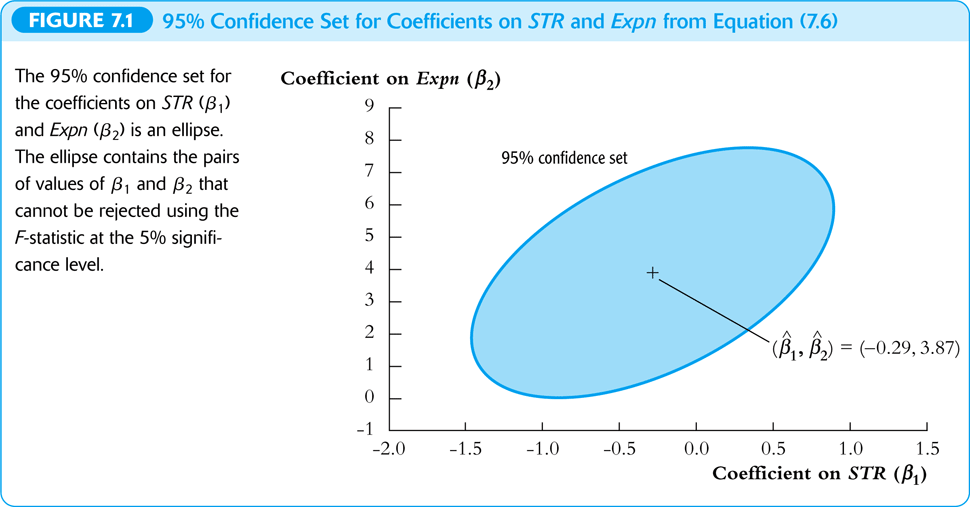
\includegraphics[width=.9\linewidth]{img/fig-7-1.png}
\caption{\label{fig:org24b6cab}
95\% Confidence Set for Coefficients on STR and Expn}
\end{figure}


\section{Model specification for multiple regression}
\label{sec:org108c6b0}

\subsection{Omitted variable bias in multiple regression}
\label{sec:org2415f05}

Omitted variable bias is the bias in the OLS estimator that arises
when one or more included regressors are correlated with an omitted
variable.

For omitted variable bias to arise, two things must be true:
\begin{enumerate}
\item At least one of the included regressors must be correlated with the
omitted variable.
\item The omitted variable must be a determinant of the dependent
variable, \(Y\).
\end{enumerate}

With omitted variable bias, the least square assumption \(E(u|X) = 0\)
does not hold any more. The OLS estimator \(\hat{\beta}\) is biased
however large the sample size is.


\subsection{The problem of the assumption of \(E(u|X) = 0\) and control variables}
\label{sec:orgcab33aa}

The assumption of \(E(u|X) = 0\) ensures that the estimated coefficients
on all included regressors are unbiased and consistent. However, this
assumption is too strong to be completely realized in practice. So we
have to make a compromise between the ideal situation and reality.

What we can do is that we divide all regressors into two groups:
\begin{itemize}
\item One group consists of regressors whose causal effects on \(Y\) are our
research interest so that we want unbiased estimates of these
coefficients.
\item Another group consists of regressors whose causal effects on \(Y\) are
not our focus. But if we omit them, we would risk making omitted
variable bias in the coefficients that we do care.
\end{itemize}
The regressors in the latter group are called \textbf{control
variable}. Moreover, we use an assumption that is weaker than the
assumption of \(E(u|X)=0\) to ensure that the estimated coefficients on
the regressors in the first groups are unbiased, maintaining the causal
implication that we want.


\subsection{The role of control variables in multiple regression}
\label{sec:org0c4463a}

\subsubsection*{Definition}
\label{sec:org0fc4be8}

A control variable \(W\) is a variable that is correlated with, and
controls for, an omitted causal factor in the regression of Y on X,
but which itself does not necessarily have a causal effect on Y.

A control variable is not the object of interest in the study; rather
it is a regressor included to hold constant factors that, if
neglected, could lead to the estimated causal effect of interest to
suffer from omitted variable bias.

\subsubsection*{The test score example}
\label{sec:org49ae3cb}

\[TestScore = \underset{(5.6)}{700.2} - \underset{(0.27)}{1.00}STR -
\underset{(0.033)}{0.122}PctEL - \underset{(0.024)}{0.547}LchPct,\,
\bar{R}^2 = 0.773 \]

Where \(PctEL=\) percent English learners in the school district,
\(LchPct=\) percent of students receiving a free/subsidized lunch.

\begin{itemize}
\item Which variable is the variable of interest? \(STR\)
\item Which variables are control variables? Do they have causal
implications? What do they control for?
\begin{itemize}
\item \emph{PctEL} probably has a direct causal effect (school is tougher if
you are learning English!).  But it is also a control variable:
immigrant communities tend to be less affluent and often have
fewer outside learning opportunities, and \emph{PctEL} is correlated with
those omitted causal variables.  \emph{PctEL} is both a possible causal
variable and a control variable.
\item \emph{LchPct} might have a causal effect (eating lunch helps learning);
it is also correlated with and controls for income-related outside
learning opportunities.  \emph{LchPct} is both a possible causal variable
and a control variable.
\end{itemize}
\end{itemize}

\subsubsection*{What makes an effective control variable?}
\label{sec:org1958dec}

What variables can we choose to include in regression as effective
control variables?  The followings are three interchangeable
statements about what makes an effective control variable:
\begin{itemize}
\item An effective control variable is one which, when included in
the regression, makes the error term uncorrelated with the variable of
interest.
\item Holding constant the control variable(s), the variable of interest
is “as if” randomly assigned.
\item Among individuals (entities) with the same value of the control
variable(s), the variable of interest is uncorrelated with the
omitted determinants of \(Y\).
\end{itemize}

Control variables need not be causal, and their coefficients
generally do not have a causal interpretation.
\begin{itemize}
\item Does the coefficient on \emph{LchPct} have a causal interpretation?  If
so, then we should be able to boost test scores (by a lot! Do the
math!) by simply eliminating the school lunch program, so that
\(LchPct = 0\). But it makes nonsense!
\end{itemize}


\subsection{Conditional mean independence}
\label{sec:org849901b}

We need a mathematical statement of what makes an effective control
variable, which is \textbf{conditional mean independence}.

Conditional mean independence says that given the control variable(s),
the expectation of \(u_i\) doesn’t depend on the variable of interest.

Let \(X_i\) denote the variable of interest and \(W_i\) denote the control
variable(s).  \(W\) is an effective control variable if conditional mean
independence holds:
\[ E(u_i|X_i, W_i) = E(u_i|W_i) \]

If \(W\) is an effective control variable, then we can use conditional
mean independence to substitute the first least square assumption
requiring \(E(u_i | X_i, W_i) = 0\).

Consider the regression model \[ Y = \beta_0 + \beta_1 X + \beta_2 W +
u \] where \(X\) is the variable of interest and \(W\) is an effective
control variable so that conditional mean independence holds. In
addition, suppose that the other least square assumptions hold. Then,
it has the following tow implications: (1) \(\beta_1\) has a causal
interpretation and (2) \(\hat{\beta}_1\) is unbiased and \(\hat{\beta}_2\)
is biased. Let's see the reasons.

\subsubsection*{\(\beta_1\) has a causal interpretation.}
\label{sec:org1ee2910}

It means that controlling for \(W\), the causal effect of \(X\) on \(Y\) is
measured by \(\beta_1\). That is, we can still interpret \(\beta_1 =
\Delta Y / \Delta X\), holding other things constant by controlling for
\(W\).

The expected change in \(Y\) resulting from a change in \(X\), holding \(W\)
constant, is:
\begin{equation*}
\begin{split}
& E(Y|X = x + \Delta x, W = w) - E(Y|X = x, W = w) \\
&= \beta_0 + \beta_1(x + \Delta x) + \beta_2 w + E(u|X = x + \Delta x, W = w) \\
&\text{ } - \beta_0 + \beta_1 x + \beta_2 w + E(u|X = x, W = w) \\
&= \beta_1 \Delta x + \left[ E(u|W = w) -  E(u|W = w) \right] \\
&= \beta_1 \Delta x
\end{split}
\end{equation*}
In the second equality, we use conditional mean independence \(E(u|X =
x + \Delta x, W = w) = E(u|X = x, W = w) = E(u|W = w)\).

\subsubsection*{\(\hat{\beta}_1\) is unbiased and \(\hat{\beta}_2\) is biased}
\label{sec:orgdb8f97f}

For convenience, suppose that \(E(u|W) = \gamma_0 + \gamma_1 W\). Thus,
under conditional mean independence, we have
\[ E(u|X,W) = E(u|W) = \gamma_0 + \gamma_1 W \]
Let \(v = u - E(u|W)\) so that
\[E(v|X, W) = E(u|X,W) - E(u|W) = 0 \]
Then, it follows that
\[ u = E(u|X,W) + v = \gamma_0 + \gamma_1 W + v \text{ . } \]

Then, the original model \(Y = \beta_0 + \beta_1 X + \beta_2 W + u\)
becomes
\begin{equation}
\begin{split}
Y &= \beta_0 + \beta_1 X + \beta_2 W + \gamma_0 + \gamma_1 W + v \notag \\
&= (\beta_0 + \gamma_0) + \beta_1 X + (\beta_2 + \gamma_1) W + v \notag \\
&= \delta_0 + \beta_1 X + \delta_2 W + v
\end{split}
\end{equation}
where \(\delta_0 = \beta_0 + \gamma_0\) and \(\delta_2 = \beta_2 +
\gamma_2\).

For the new model \(Y = \delta_0 + \beta_1 X + \delta_2 W + v\), we can
conclude as follows.
\begin{itemize}
\item The new model satisfy \(E(v|X,W) = 0\) so that the OLS estimator of
\(\delta_0, \beta_1, \text{ and } \delta_2\) are unbiased.
\item The estimated coefficients in the original model are actually
\(\hat{\beta}_1\) and \(\hat{\delta}_2\), which we know that
\(E(\hat{\beta}_1) = \beta_1\) and \(E(\hat{\beta}_2) = \delta_2 \neq
  \beta_2\) in general.
\end{itemize}

\subsection{Model specification in theory and in practice}
\label{sec:orgde2fce2}

In theory, when data are available on the omitted variable, the
solution to omitted variable bias is to include the omitted variable
in the regression. In practice, however, deciding whether to include a
particular variable can be difficult and requires judgment.

The following steps are advocated to set up a regression model:
\begin{enumerate}
\item a  base set of regressors should be chosen using a
combination of expert judgment, economic theory, and knowledge of
how data were collected. The regression using this base set of
regressors is referred to as a \textbf{base specification}. This step
involves the following consideration:
\begin{enumerate}
\item identifying the variable of interest.
\item thinking of the omitted causal effects that could result in omitted
variable bias.
\item including those omitted causal effects if you can find relevant
variables. If you can’t, include variables that are correlated
with them as control variables. The control variables are
effective if the conditional mean independence assumption
plausibly holds.
\end{enumerate}
\item Specify a range of plausible \textbf{alternative model specifications},
which include additional candidate variables.
\begin{enumerate}
\item If the estimates of the coefficients of interest are numerically
similar across the alternative specifications, then this
provides evidence that the estimates from your base
specification are reliable.
\item If the estimates of the coefficients of interest change
substantially across specifications, this often provides
evidence that the original specification had omitted variable
bias.
\end{enumerate}
\item Use test statistics to judge a model specification
\begin{enumerate}
\item Use \(R^2\) and \(\bar{R}^2\) to see the overall goodness of fit of
a model specification. Caution: a high \(R^2\) or \(\bar{R}^2\) does
not mean that you have eliminated omitted variable bias. Neither
does a high \(R^2\) or \(\bar{R}^2\) mean that the included
variables and the model as a whole are statistically
significant.
\item Use t-statistic to check the significance of individual
coefficients, and use F-statistic to check the overall
significance of the model as a whole. That is, use F test for
\[H_0:\, \beta_1 = \beta_2 = \cdots = \beta_k = 0 \]
\end{enumerate}
\end{enumerate}


\section{Analysis of the test score data set}
\label{sec:org8f2fa5c}
The complete regression results are formally reported in Table 7.1.

\begin{figure}[!ht]
\centering
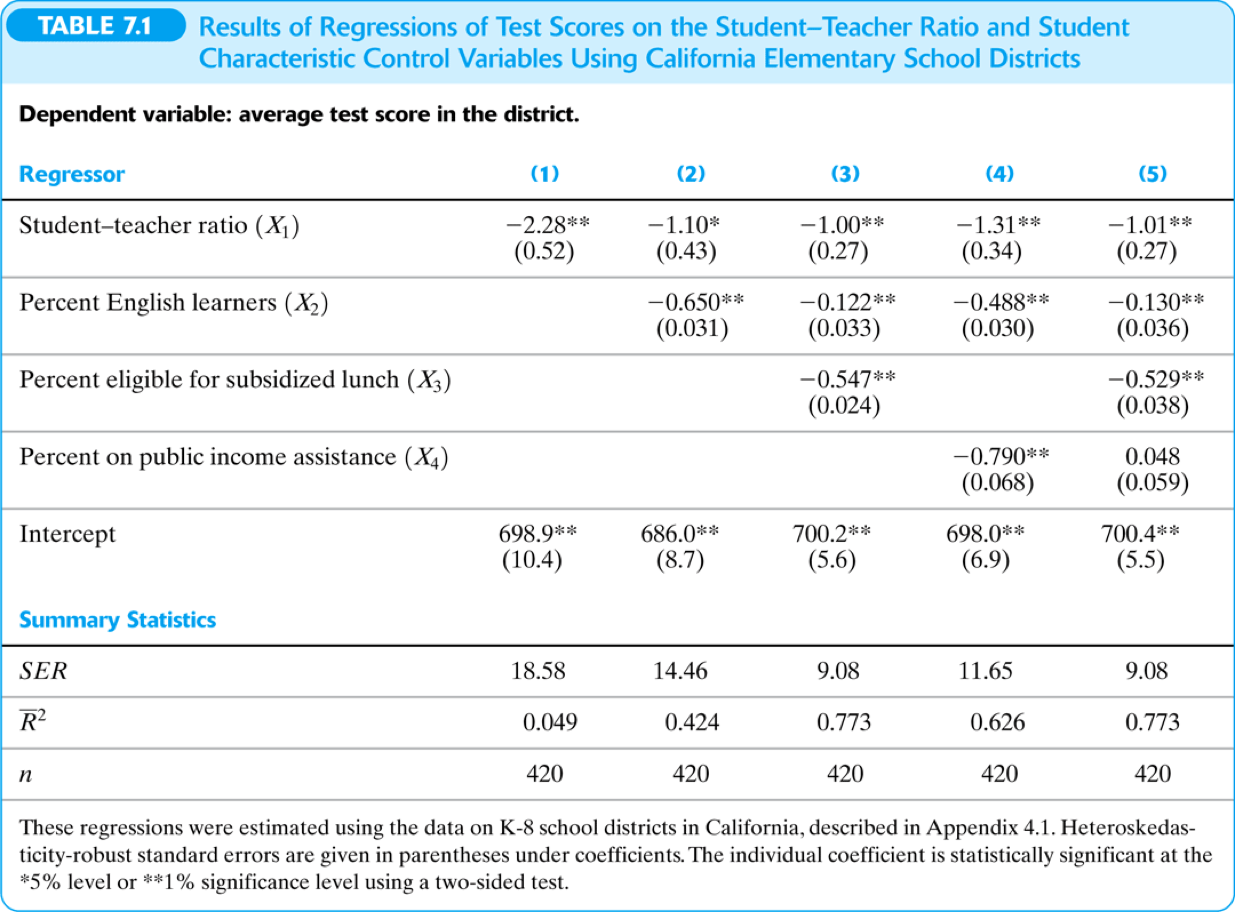
\includegraphics[width=1.0\textwidth]{img/tab-7-1.png}
\end{figure}
\end{document}